\documentclass{article}
\usepackage[utf8]{inputenc}
\usepackage{graphicx}
\title{Data Analysis Project 1}
\author{Buz Galbraith }
\date{November 2022}

\begin{document}

\textbf{Buz Galbraith,DS GA: 1000 Data Analysis Project 1}

\subsection*{General assumptions}
\small{
Before answering specific questions I am going to state some general assumptions. Firstly, I used element wise removal of missing values for all analysis. 
This naturally also assumes that not watching one movie is independent of another, I would argue that this assumption is irrelevant to all questions except 10, as we are not trying to understand how watching one movie effects another but instead how other factors effect movie watching habits. Next I only conducted non-parametric tests I would argue this is reasonable as ratings data is ordinal and thus means are not meaningful.  }  

\section*{Mann-Whitney U Test Questions}
All questions in this section were approached with the Mann-Whitney U test, so I will outline the assumptions that are common to them all and explain the specifics in each question's subsection. The Man Whitney U test applies to data where the mean is not meaningful, which holds for comparisons of movie ratings that are not asking specifically about the distribution. Further, all of these questions are only comparing at most two groups at a time, thus the KS test in unsuitable for this application. 
\subsection*{Question 1}
For this question I conducted a one way Mann-Whitney U test comparing popular and unpopular movies. As can be observed by figure 1 in the appendix this data has outliers so the median is going to be more descriptive than the distribution. Running this test yields a p value bellow ${\alpha}$, thus we reject our null hypothesis that movies which are more popular are likely to be rated more highly due to chance alone. %There is a fair question of if those who watch both unpopular movies and popular movies, could be more into film, and if they might rate movies diferently than %
\subsection*{Question 2}
To answer this question ran a two-way Mann-Whitney U test comparing older and newer movies. Additionally we can see by looking at figure 2, the samples have fairly high variance, so the Mann-Whitney is further a good choice as it is robust to outliers.  Running this test yields a p value bellow $\frac{\alpha}{2}$, thus we reject our null hypothesis that the deference in the ratings of newer and older movies is due to chance alone. A major limitation of this analysis could be temporal bias. Many people only watch movies when they come out, so perhaps people could rate movies that they have seen more recently higher than those that they saw a long time ago. 
\subsection*{Question 3}
To answer this question I ran a two-way Mann-Whitney U test comparing males who have watched Shrek to females who have watched Shrek. Again we can see by looking at figure 3 that the medians appear to be substantially different between male and female Shrek viewers. Here it is worth noting that only $78$ females, watched Shrek while $241$ males watched Shrek. Running this test yields a p value bellow $\frac{\alpha}{2}$, thus we reject our null hypothesis that the deference in male and female ratings of Shrek may be due to chance alone. It is worth noting that this analysis may be limited by the fact that only 7$\%$ of females watched Shrek, so our degrees of freedom are relatively limited. 
\subsection*{Question 4}
For this question I ran two-way Mann-Whitney U Tests comparing male and female viewers for each of the 400 movies, then found the ratio of those that had significant alpha values over the total number of tests run. I found that about $10.75\% $ seem to be enjoyed differently by men and woman. A natural draw back of this is alpha inflation, as I ran the same test 400 times, and did not account for how this may cause my false positive rate to increase. I would argue this may be OK, as due to the large sample size, our power is generally quite high.


\subsection*{Question 5}
For this question I ran a one sided Mann-Whitney U Test comparing on people with siblings who had watched The Lion King and people with out siblings who had watched The Lion King. As can be seen by looking at figure, 5 the distributions of those with and with out siblings do not seem radically different with high medians and low outliers. Running this test, we got a P value well above $\alpha$, so we fail to reject the null hypothesis that only children do not enjoy the lion king more than those with siblings.
\subsection*{Question 6}
For this question I ran a two sided Mann-Whitney U Test comparing groups of viewers who had siblings to those who did not for each of the 400 movies then found the ratio of those that had significant alpha values over the total number of tests run. I found that about $0.75\% $ seem to be enjoyed differently by those with and without siblings. Again we should be concerned about alpha inflation, as I ran the same test 400 times, and did not account for how this may cause my false positive rate to increase. I would argue however that as alpha inflation is only likely to increase our false positive rate, the general notion that it is rare for movies to effect those with or with out siblings differently likely still holds.


\subsection*{Question 7}
For this question I ran a one way Mann-Whitney U Test comparing groups of viewers who had seen the Wolf of Wall Street and prefer movies alone to those who had seen the movie and prefer watching movies socially. Here it is worth noting that we have many more observations of those who prefer to watch movies socially, than those who prefer to watch movies alone, however in both groups about $65\%$ of people who responded had seen the Wolf of Wall Street and the Mann-Whitney U Test does not require equal sample size so this should be fine. Additionally as can be seen by looking at figure 7, the distributions of each group appear to be quite similar. This is corroborated by running the Mann-Whitney U Test, which yields a p value larger than $\alpha$. Thus we fail to reject that weather or not you prefer to socially watch movies does not influence your opinion on the Wolf of Wall Street.   

\subsection*{Question 8}

For this question I ran a two sided Mann-Whitney U Test comparing groups of viewers prefer watching movies alone to those who prefer watching movies with others for each of the 400 movies then found the ratio of those that had significant alpha values over the total number of tests run. I found that about $1.5\% $ of movies seem to be enjoyed differently by by those who like to watch movies socially and those who prefer to watch movies alone. Again we should be concerned about alpha inflation, as I ran the same test 400 times, and did not account for how this may cause my false positive rate to increase. I would argue however that as alpha inflation is only likely to increase our false positive rate, the general notion that a social watching effect is rare, likely still holds though.
\section*{Non-U test Questions}
\subsection*{Question 9}
Here we are being asked to compare two distributions thus we are going to want to use the KS test. Again we did element wise missing value removal. This is unlikely to matter however as the KS test does not assume the samples are of the same size. Further we are looking at CDFs, so I don't think removing individual values should effect the overall trend of population density. As can be seen by figure 9, there is fairly large D between CDFs of the two graphs. this is corroborated by the test which yields a p value smaller than $\alpha$ and thus we reject the null hypothesis that the difference in distributions is due to chance alone.   
\subsection*{Question 10}
To solve this question we need to use the Kruskal-Wallis test. This makes sense as we are comparing multiple movies within a franchise to one another. Further as stated above ratings data is ordinal so we don't want to use tests that rely on the mean. This question does however, very seriously call into question if one can element wise drop missing values. Namely as watching one movie in a franchise is not independent from another. I would however argue, that what we are entrusted in generally is if how the movies within a series are reviewed changes over the course of a series, not how individuals who watched each movie rated them. So the opinions of those who only watched one film are still rel event for analysis. So we ran 1 Kruskal-Wallis test on the films of each franchise, and counted the number that had a significant change in quality one way or another. We found that $87.5\%$ of franchises did have this quality change. 

\subsection*{Extra Credit}
I thought an interesting question could be, is there a difference in responses for values of 'The emotions on the screen "rub off" on me - for instance if something sad is happening I get sad or if something frightening is happening I get scared' between males and females? I firstly dropped, all rows that did not correspond to a male or female, as well as all males or females that did not respond to the prompt. I think this was reasonable, as there were few individuals who did not identify as male or female, and $98\%$ of participants responded to the question of if emotions rubbed off on them, so we are unlikely to be losing much data. Looking at the distributions in figure 7, it seems like females have a higher mean, and are skewed downward, while males have a lower mean and overall high variance.  Running a two sided Man Whitney U test, resulted in a p-value lower than $\alpha/2$ thus there is reason to believe that male and female viewers had different emotional reactions to movies.  


\newpage\section*{Appendix}

\begin{figure}
\label{fig:foo}
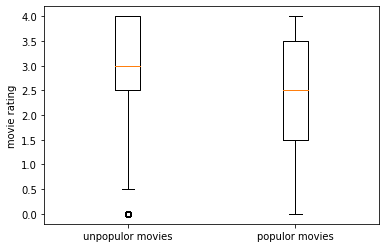
\includegraphics[width=15cm]{data analysis project 1/boxplot question 1..png}
\caption{Box plot of popular and unpopular movies}
\end{figure}
\begin{figure}
\label{fig:foo}
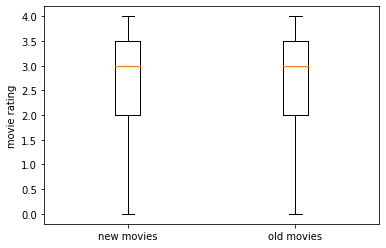
\includegraphics[width=15cm]{data analysis project 1/boxplot question 2.png}
\caption{Box plot of New and Old movies}
\end{figure}


\begin{figure}
\label{fig:foo}
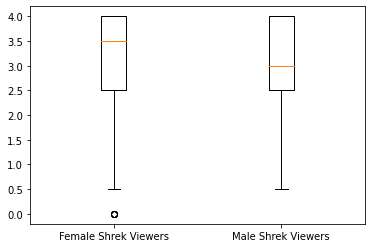
\includegraphics[width=15cm]{data analysis project 1/boxplot question 3.png}
\caption{Box plot of Female and Male Shrek Viewers}
\end{figure}

\begin{figure}
\label{fig:foo}
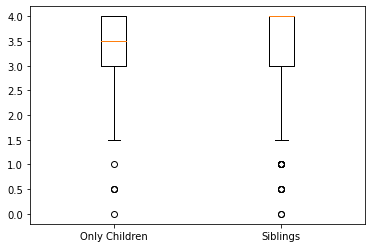
\includegraphics[width=15cm]{data analysis project 1/boxplot question 5.png}
\caption{Box plot of only children versus those with siblings}
\end{figure}

\begin{figure}
\label{fig:foo}
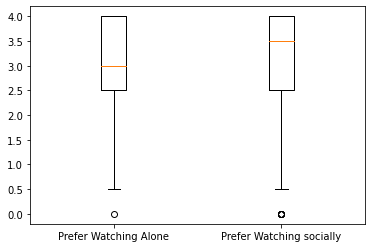
\includegraphics[width=15cm]{data analysis project 1/boxplot question 7.png}
\caption{Box plot of those who prefer watching alone versus socially}
\end{figure}


\begin{figure}
\label{fig:foo}
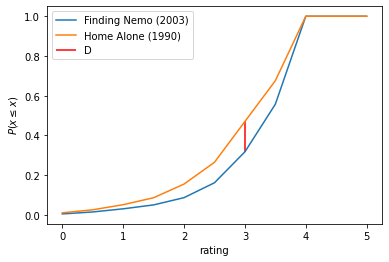
\includegraphics[width=15cm]{data analysis project 1/boxplot question 9.png}
\caption{distribution of Finding Nemo ratings versus Home Alone ratings}
\end{figure}


\begin{figure}
\label{fig:foo}
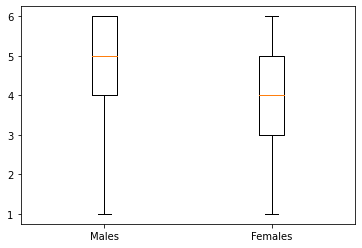
\includegraphics[width=15cm]{data analysis project 1/extracredit boxplot.png}
\caption{distribution of response to "movies emotionally effect me plot" by gender}
\end{figure}




\end{document}
